\documentclass{acm_proc_article-sp}
%\documentclass[10pt, conference, compsocconf]{IEEEtran}

% From ASIACCS'13 CFP
% Submissions must be written in English, and must be at most 10 pages
% excluding the bibliography and well-marked appendices, and at most
% 12 pages overall.

\usepackage{listings}
\usepackage{url}

\usepackage{amssymb}
\usepackage[usenames]{color}
\definecolor{lightred}{rgb}{1,0.8,0.8}
\newcommand{\todo}[1]{\colorbox{red}{\textcolor{white}{\sffamily\bfseries\scriptsize TODO}} \textcolor{red}{#1} \textcolor{red}{$\blacktriangleleft$}}


\title{Crossing Origins by Crossing Formats}

\begin{document}


% \author{\IEEEauthorblockN{Jonas Magazinius} 
% \IEEEauthorblockA{Department ofComputer Science\\ 
% Chalmers University of Technology\\ 
% Gothenburg, Sweden\\
% jonas.magazinius@chalmers.se} 
% \and 
% \IEEEauthorblockN{Billy Rios} 
% \IEEEauthorblockA{dept. name of organization\\ 
% name of organization, acronyms acceptable\\ 
% City, United States of America\\ 
% Email: name@xyz.com} 
% \and 
% \IEEEauthorblockN{Andrei Sabelfeld} 
% \IEEEauthorblockA{Department of Computer Science\\ 
% Chalmers University of Technology\\ 
% Gothenburg, Sweden\\ 
% andrei@chalmers.se} 
% }

\maketitle



\begin{abstract}
 In a heterogeneous system like the web, information is
exchanged between components in versatile formats. A new breed of attacks is on
the rise that exploit the mismatch between the expected and provided content.
% 
This paper identifies the root cause of a large class of attacks: \emph{polyglots}. 
A polyglot is a program that is valid in multiple programming languages. Polyglots allow
multiple interpretation of the content, providing a new space of attack vectors.
%
We characterize of what constitutes a dangerous format in the web setting and
identify particularly dangerous formats, with PDF as the prime example. We
demonstrate that polyglot-based attacks on the web open up for insecure
communication across Internet origins. 
%
The paper presents novel attack vectors that infiltrate the trusted
origin by \emph{syntax injection} across multiple languages and by
\emph{content smuggling} of
malicious payload that appears formatted as benign content. The
attacks lead to both \emph{cross-domain leakage} and \emph{cross-site
  request forgery}.
%
We perform a systematic study of
PDF-based injection and content smuggling attacks. We evaluate the current
practice in client/server content filtering and PDF readers for polyglot-based
attacks, and report on vulnerabilities in the top 100 Alexa web sites. Our
recommendations for protective measures on server side, in browsers, and in content
interpreters (in particular, PDF readers) show how to mitigate the attacks.
\end{abstract}


% \begin{IEEEkeywords}
% Web Security; Polyglot; Injection; Cross-domain.
% \end{IEEEkeywords}








%1 pages
\section{Introduction}
\label{sec:intro}
Web application security is concerned with protecting information as
it is manipulated by web applications. This is an important area
because ``attacks against web
applications constitute more than 60\% of the total attack attempts
observed on the Internet''~\cite{SANS09}.

\paragraph{Internet origins at stake}
The different trust domains
correspond to different Internet origins. A major goal for web
application security is preventing undesired communication across
origins. 
%
With the goal of separating information from the different origins,
today's browsers enforce the \emph{same-origin policy} (SOP). SOP
only allows access between two documents if they share the
origin. In addition, a document can only directly communicate with the
server from which it originates.

\paragraph{Classical cross-domain attacks}
There are several classes of cross-domain attacks that circumvent SOP.
The OWASP top 10 list~\cite{OWASP:top10:2010} places \emph{injection}
and \emph{cross-site scripting} (XSS) attacks as two top security
risks for web applications.
%
A classical XSS attack injects a malicious script in the context of a
trusted origin. This opens up opportunities for leaking sensitive
information that users might have in the context of the trusted origin
such as cookies, personal information, and session tokens.

XSS attacks are relatively well understood by researchers and
developers~\cite{XSSED}. Known defense include various
flavors of \emph{sanitization} on server side and the
\emph{content security policy}~\cite{CSP1.0} (CSP) on client side. Sanitization
is often performed by the server to filter possibly malicious input data
before it is used in the generated web pages. Content security policy puts
requirement on the structure of the document and the origins of the
scripts that are included by web pages.

\paragraph{Crossing origins by crossing formats}
This paper identifies a new breed of attacks and its root cause:
\emph{polyglots}. 
%
A polyglot is a program that is valid in multiple programming languages.
%
In a heterogeneous system like the web, information is exchanged
between components in versatile formats.
%
This gives rise to attacks that exploit the mismatch between the
expected and provided content.
%

Polyglots allow
multiple interpretation of the content, providing a new space of attack vectors.
We present novel attack vectors that are based on (i)
\emph{syntax injection} that 
operate across multiple languages and on (ii) \emph{content smuggling} that supply
malicious payload that appears formatted as benign content. The
attacks lead to both \emph{cross-domain leakage} and \emph{cross-site
  request forgery}.

The existing defense mechanisms fall short to prevent these attacks
from achieving cross-domain communication. 
On the server side, santization is specific to the target language of
the web application. Sanitizing unexpected formats is typically not considered.
On the client side, CSP
has no effect unless the content is interpreted as HTML. This opens up
opportunities for attacks that are based on other formats.

First steps in exploiting the formats in the context of the web have
been by researchers. Two noteworthy examples are GIFAR~\cite{Brandis:GIFAR} and
cross-origin CSS attacks~\cite{Huang+:CCS10} (Section~\ref{sec:related}
discusses further related work). 
%
GIFAR is based on polyglots that combine the GIF and JAR (Java
archive) formats. The former is used as benign and the latter as
malicious to bypass SOP.
%
Cross-origin CSS attacks inject fragments of CSS code into an existing
web page to extract information from the existing web page.
%
The paper is the first to perform a systematic study of polyglot
attacks.
We characterize of what constitutes a dangerous format in the web setting and
identify particularly dangerous formats, with PDF as the prime example. We
demonstrate that polyglot-based attacks on the web open up for insecure
communication across Internet origins. We perform a systematic study of
PDF-based injection and content smuggling attacks. 


\paragraph{Evaluation and mitigation}
We evaluate the current
practice in client/server content filtering and PDF readers for polyglot-based
attacks, and report on vulnerabilities in the top 100 Alexa web sites. Our
recommendations for protective measures on server side, in browsers, and in content
interpreters (such as PDF readers) show how to mitigate the attacks.

\paragraph{Contributions} The paper makes the following contributions:
\begin{itemize}
\vspace*{-.6cm}
\item Identification of polyglot attacks, a new breed of attacks for
  crossing origins by crossing formats;
\vspace*{-.2cm}
\item Characterization of the necessary ingredients for polyglot attacks
\vspace*{-.2cm}
\item Highlighting the PDF format as a particularly exposed format for
  polyglot attacks;
\vspace*{-.2cm}
\item Novel confidentiality and integrity attack vectors, based on syntax 
  injection and content smuggling;
\vspace*{-.2cm}
\item Evaluation of the current filtering mechanisms, browsers, and PDF
  filters for vulnerabilities; and
\vspace*{-.2cm}
\item Mitigation for the server, client, and PDF readers.
\end{itemize}


\paragraph{Overview}
The paper is organized as follows. 
%
Section~\ref{sec:cross} explains the concept of crossing origins by
crossing formats, identifies necessary ingredients, and provides
attack scenarios.
%
Section~\ref{sec:vuln} focuses on the PDF format and describes
concrete vulnerabilities and attacks.
%
Section~\ref{sec:eval} evaluates the current practice in client/server
content filtering and PDF readers and report on vulnerabilities in the
top 100 Alexa web sites.
%
Section~\ref{sec:mit} suggests mitigation for servers, clients, and
PDF readers.
%
Section~\ref{sec:related} discusses the related work.
%
Section~\ref{sec:conc} concludes and outlines future work.

%3 pages
\section{Crossing origins by crossing formats}
\label{sec:cross}
% Describe how the attacks lead to same-origin policy bypass.

This section describes how formats can be crossed and how that can be abused 
to cross origins by circumventing the same-origin policy. We begin by 
generalizing the problem of crossing formats to \emph{polyglots} and then describe the  
characteristics of a malicious polyglot. From that we derive two attack vectors and 
show how previous work on the subject relate to these vectors.

\subsection{Crossing origins}
\label{sec:cross-origin}

By crossing origins we mean being able to request and access content
which is normally restricted under the same-origin policy. 
Recall that SOP only allows two documents accessing each others'
content and resources if they share the origin. Similarly,
a document can only directly communicate with the server from which it originates. 
This is not to be confused with \emph{cross-origin resource sharing} (CORS)~\cite{w3-cors}, which is an 
intentional relaxation of SOP.

While there are exceptions to this policy, e.g. images, scripts, and style sheets 
are allowed to be included as resources across origins, access to these resources is 
restricted to prevent information leaks. As an example, the including 
document is prevented from accessing the image data of images loaded across 
origins. 

Not all elements are as carefully restricted from information leaks as images. 
Scripts loaded across origins become part of the document and inherit the 
origin of the including document, which allows the script to communicate with the 
server from which the \emph{document} originates. Such scripts are also able to interact 
with the document, e.g. by adding nodes, which in turn require new content to be 
requested. Since these requests are not restricted by SOP, this creates a side 
channel that permits cross-origin information leakage. At the same time, the including document
is prevented from inspecting the source of the script and can only observe the public 
side-effects that the script produce as it is executed.

Other examples of problematic elements include the \emph{object} and
\emph{embed} tags. These 
tags allow inclusion of resources that might require a 
plug-in to run. As with images, the content handled by the plug-in retains its origin, 
but the browsers are forced to rely on the plug-ins to employ correct security 
measures to prevent information leaks. The plug-in is selected based on the MIME-type of the content, but
because the server delivering the content might not be able to determine its
format, the \emph{object} tag allows a developer to set the type-attribute to guide the
browser in which plug-in to run. When the type attribute is used, the
corresponding plug-in is run regardless of which MIME-type the server returns
and it is up to the plug-in to respond to and handle the content it is served. While the containing page is restricted 
from directly accessing the content handled by the plug-in, a number of plugins provide 
an API for interacting with the plug-in and the data. As we will show, this can lead to 
to cross-origin information leaks.


\subsection{Crossing formats}

% What and how?

A polyglot is perhaps most commonly known as a person who speaks several
languages. However, the term
is widely used in several scientific fields. In computer science, a \emph{polyglot} is
a program that is valid in multiple programming languages. In this paper we use
a broader definition of a programming language, not limited to code meant for
compilation to machine code or scripting languages, but extended to any format
that requires interpretation before rendering.

A polyglot is composed from various constructs that are either common between
languages; or constructs that are language specific, but carrying different
meaning in each language. To maintain validity across languages, one must ensure
that language specific constructs are not interpreted by other languages. This
is often accomplished by hiding the parts of the code specific to one language,
in parts interpreted as comments or plain text of another.

Certain languages are particularly suitable for creating polyglots. These
languages either have a lot of constructs in common with other languages, such
as the C language, or are defined such that the parser ignores that which it cannot
interpret, such as HTML. The latter allows for ample opportunity to hide
any code specific to another language, as long as there is no overlap with the
syntax of the first language.


%\paragraph{Malicious polyglots}

% What is a malicious polyglot? - One part benign one part malicious

A malicious polyglot is composed of two formats where one is benign in nature and the other
contains a malicious payload. 
% Characteristics of a malicious polyglot
The benign format is a widely accepted format with the capability 
of hiding arbitrary data, e.g. an image with comment fields. The malicious 
format has additional capabilities, such as scripting.
% Under what circumstances can a polyglot be malicious
This kind of polyglot can be used for malicious purposes when there is a difference between
the expected run-time context and the actual context it is executed in. 
In the expected context the content is interpreted as the 
benign format. In the actual context, however, the content is coerced to be 
interpreted as the malicious format containing the payload.

Even if a verification process exists, it verifies that the content is valid 
in the expected context. Due to the nature of the polyglot, the content is 
verified as valid and benign, but subsequently the malicious
content is executed.

Coercing content to be interpreted
as a different type can be accommodated in the context of the web. 
If the content is loaded using an \emph{image} tag it will be interpreted 
as an image, if a \emph{script} tag is used it will be interpreted as a script. Some 
tags even let the developer decide which type to interpret the content as. 
To prevent abuse, the browsers employ content-type 
sniffing for certain content-types, a practice which has historically led to 
security issues.

Barth et al.~\cite{Barth+:SP09} define \emph{chameleon} documents, 
in which a benign file type crossbred with malicious HTML content. The document 
is crafted in such a way that the content-sniffing algorithm used in the browser 
will detect the content type as HTML. The paper proceeds to 
describe how an attacker can create a 
\emph{chameleon} document, that is valid PostScipt, but will be identified as HTML.
This issue allows exploitation when there is a mismatch between a websites 
content validation filter and the browsers content-sniffing algorithm.

In literature we find, apart from chameleons, other names for similar,
related concepts. Brandis~\cite{Brandis:GIFAR} refer \emph{GIFAR} 
attacks, based on one of the early instances of attacks based on 
GIF/JAR polyglots. 
Sundareswaran et al.~\cite{Sundareswaran:Squicciarini:CEAS10,Sundareswaran:Squicciarini:SecureComm10}
discuss GIFAR-related attacks as a form of \emph{content repurposing} attack. 
In this paper the term content smuggling is used as it best represent 
how a polyglot can infiltrate an origin.


\subsection{Scenario}


The victim in these scenarios is an authenticated user of a targeted vulnerable website, \emph{vulnerable.com}. 
The target is infiltrated by the attacker, manipulating the website to serve polyglot content. Vulnerable.com serves the polyglot content as the benign content type, harmless to the victim. 
At a certain point, while still authenticated to vulnerable.com, 
the victim unsuspectingly visits the attackers malicious website, \emph{attacker.com}.
The attacker.com website embeds the polyglot content from vulnerable.com, but
coerces the browser to interpret it as the malicious content type. 
The capabilities of the malicious format determine the 
severity of the consequences of exploitation. 

Two attacker-centric components requires special attention, the infiltration of 
an origin and the exploitation of an infiltrated origin.
%In this situation, the same-origin policy is intended to prevent cross-origin 
%interaction.

\begin{figure}[h!]
  \center
  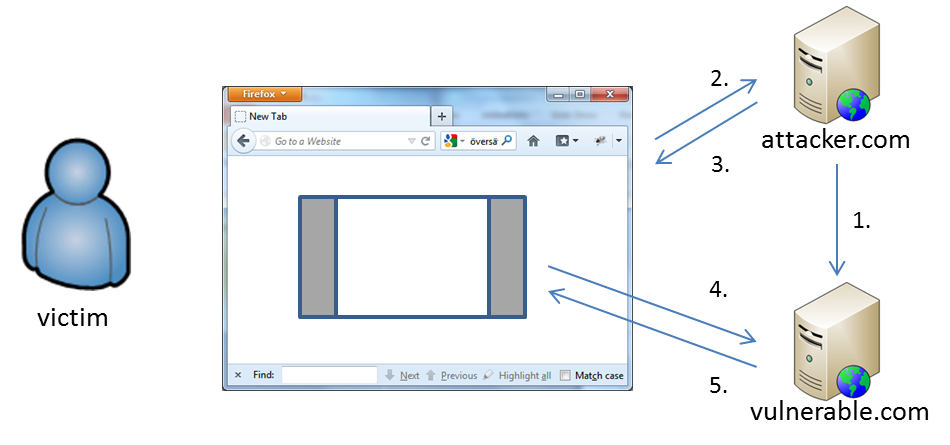
\includegraphics[width=0.49\textwidth]{scenario.png}
  \caption{Overview of the scenario}
  \label{fig:scenario}
\end{figure}

\subsection{Infiltrating an origin}

Two vectors for infiltrating an origin has been identified, via syntax 
injection, or content smuggling. 

\paragraph{Syntax injection}

In a cross-site scripting attack, a HTML document is composed from input 
containing fragments of HTML syntax, causing the execution of attacker supplied 
script code. Similarly, in a syntax injection attack the vulnerable target will 
compose content from attacker controlled input containing syntax of a foreign 
format, thereby creating a polyglot. 
%
The target is assumed to employ server-side cross-site scripting sanitization. Hence, for the attack to be successful, the input must 
bypass this sanitization. The sanitization filter will remove or encode 
problematic characters, based on the context of the web application. In a polyglot attack
the injected format would pose as a new context, unknown to the filter. Chances are that the 
key elements of the injected format will pass the filter unaltered. 
The polyglot content can
be interpreted as either the benign original format or the
malicious attacker-supplied format. 
%

%As an example the
%same-origin policy allows a \emph{script} tag in one document to include JavaScript of
%another origin and execute it in the origin of the document. If an attacker is
%able to inject an HTML document with JavaScript syntax in such a way that it
%became valid JavaScript, the attacker can include the document across origins
%via a \emph{script} tag and extract its content, thereby circumventing the same-origin
%policy.

%The document in Listing \ref{lst:html-js}, is both
%malformed but valid HTML and valid JavaScript in browsers that support
%EcmaScript for XML (E4X). \todo{ref} The
%document can be included as a script in another document and the secret can be
%extracted from variable x. 
%This implies that if an attacker is able to inject
%HTML syntax into a document, closing all previously open tags and
%opening all subsequently closed tags,
%then information can be extracted across origins.
%The injected syntax in the listing is illustrated by highlighting.

%This attack has been suggested as a potential way to bypass Content Security
%Policy~\cite{Heyes:CSP}. As E4X is only supported in the SpiderMonkey JavaScript
%engine, used in Firefox, this limits the exploitability of this example. However,
%this is an unlikely scenario to use JavaScript as the injected format
%because HTML characters are typically escaped by content
%filters. 

Previous work documents instances of polyglot attacks based on syntax injection.
Huang et al.~\cite{Huang+:CCS10} describe a cross-origin \emph{cascading style-sheet} (CSS) attack. This 
attack injects fragments of CSS syntax in a HTML 
document, thereby making it a HTML/CSS polyglot. The error-tolerant parsing of 
style sheets allow the polyglot to parsed as valid CSS. The capabilities of CSS 
provide trivial cross-origin leakage. The paper proposes a defense technique which has been
adopted by all major browsers, which implies that the attacks outlined in their paper are now ineffective.
Instead,
Section
\ref{sec:vuln} will show practical attacks based on other formats.



%\definecolor{lightgray}{gray}{.8}
%\begin{lstlisting}[label=lst:html-js, caption=HTML / E4X Polyglot, escapechar=*]
%<html><body>
%Hello *\colorbox{lightgray}{$<$/body$><$/html$>$;x=$<$html$><$body$>$}*!
%Your secret is 'safe with me'.
%</body></html>
%\end{lstlisting}


\paragraph{Content smuggling}
The vulnerable target of a polyglot attack based on content smuggling lets 
users to submit files to the service which are then served under the origin of 
the service. Examples of such services are file sharing services, image databases, 
social networks or job broker services. Such a service 
accepts a limited set of file-types, and the files are verified to
be of one of these types, e.g. an image, before being served to the end
user. By submitting a polyglot to such a service, an attacker can trick the
service into serving malicious content under the origin of the service. The
service will verify the file, assuming that it is of the benign format, but once
the content is served an attacker can coerce the content to be interpreted as
the malicious format.

The GIFAR attack is a polyglot attack based on content smuggling. In this attack 
a benign GIF-image and a malicious JAR-file is combined to create a GIF/JAR 
polyglot. By submitting the combined GIFAR to a service, the attacker can 
execute a Java applet under the origin of the targeted service. The Java runtime 
has been updated to prevent this kind of abuse.
Instead,
Section
\ref{sec:vuln} will show practical attacks based on other formats.


\subsection{Exploiting the infiltrated origin}

The consequences of exploiting an infiltrated origin depend on the capabilities 
of the format used. These consequences span from forging requests to the vulnerable website,
abusing the credentials of the victim, to extracting sensitive information about the user that is
stored on the vulnerable website.

\paragraph{Cross-site request forgery}

If the format has the capability of issuing requests, that includes the victims 
credentials, within the boundaries of the SOP, then this constitutes a 
\emph{cross-site request forgery} (CSRF) attack. Websites protect against these attacks by 
generating a token with each response that has to be included in the subsequent 
request. However, if the format also have the capability of reading the response 
the issued request, it can extract the token and thereby circumvent the CSRF 
protection.

\paragraph{Cross-origin leakage}

If the format also has the capability of communicating with the attacker, then 
the attacker can sensitive user information and leak it across origins. If the 
format is not restricted by the SOP, it can communicate directly with the 
attackers server. Otherwise, if the format can interact with the document that 
embeds the polyglot, the communication could be tunneled through this channel.






%\subsection{Syntax injection}






%For this attack to be successful certain requirements needs to be fulfilled.
%\begin{itemize} 
%	\item The original content must embed external information under the 
%	control of the attacker. 
%	\item The user-supplied content must circumvent any validation or 
%	filtering. 
%	\item There must exist a way of coercing the resulting polyglot to be 
%	interpreted as the malicious format. 
%	\item The malicious format must have capabilities that are restricted or 
%	missing in the benign format.
%\end{itemize}

% Scenarios

%Much like a cross-site scripting attack, we consider a scenario where a
%website serves documents which are based upon user-supplied information.

%The same-origin policy is intended to prevent a document from one origin from
%accessing the content of a document of another origin. 


%Consider the php-program in listing \ref{lst:php-sample}. Apart from being
%vulnerable to traditional cross-site scripting, it is vulnerable

%By requesting the site with parameter $guess=</body></html>;x=<html><body>$,
%the resulting document, 



%\subsection{Content smuggling}
% Description of attack technique 

% Building blocks

%The difference in this scenario from the previous one is in the nature of the
%vulnerability. Where in the previous scenario an existing document was injected
%to become a polyglot, this scenario targets services which allow an attacker to
%introduce new documents. As in the previous scenario, the target is a user of
%the vulnerable website.


%For this attack to be successful, certain requirements needs to be fulfilled.
%\begin{itemize} 
%	\item The service must accept and serve user-supplied files.
%	\item The service must verify the user-supplied polyglot under the 
%	assumption that it is in the benign format. 
%	\item The content is served under the same origin as sensitive user 
%	information.
%	\item There must exist a way of coercing the polyglot to be interpreted 
%	as the malicious format. 
%\end{itemize}

% Scenarios

%3 pages 
\section{Vulnerabilities and attacks}
\label{sec:vuln}

In this section we give concrete examples of the attacks described in 
Section~\ref{sec:cross}, using the PDF format as the running example. We begin
by detailing how the design decision made in the PDF-standard make it highly suitable
for creating malicious polyglots. Throughout this section Adobe Reader is the 
assumed target. A comparison between readers can be found in Section~\ref{sec:eval}.

The reader is invited to visit the test page~\cite{Test:Page:12} for
practical demonstration of the concepts from this section.

%\subsection{Concept}


\subsection{Portable Document Format}
\label{sec:format}
% Why PDF format?

The \emph{Portable Document Format} (PDF) is a widely used document format 
capable of displaying text, rendering graphics, scripting, animation and other 
dynamic content. It is a container format in the sense that it allows 
embedding of files and resources.

According to the PDF specification~\cite{PDF:ISO08} a PDF file is composed of
a header, several objects, a cross-reference section and a trailer. Listing~\ref{lst:sample-pdf} 
shows a sample of how a PDF file is structured and its elements.

\begin{lstlisting}[label=lst:sample-pdf, caption=Sample PDF file]
%PDF-1.7
1 0 obj<</Type/Catalog/Pages<<>>>>
endobj
2 0 obj<</Length 13>>stream
Sample Author
endstream
endobj
xref
0 3
0000000000 65536 f
0000000009 00000 n
0000000057 00000 n
trailer<</Root 1 0 R
	/Info<</Author 2 0 R>>
>>
startxref
118
%%EOF
\end{lstlisting}


% header
\subsubsection{Header}
The header consists of the string "\%PDF-" followed by a version number. 
The version is denoted by a 
major and a minor version number of the form "\emph{M.m}". Because the version can 
be specified elsewhere, the version number is not required to be part of the 
header.

% objects
\subsubsection{Objects}
Objects can be direct or indirect, the difference being that indirect objects 
has labels which are used for referring to the object from another object. Object 
labels are numbered and begin with the string "\emph{N n} obj", where "N" is the object number and "n" is the 
revision number. Similarly object references are of the form "\emph{N n} R".
The label is optionally ended with the keyword "endobj".

There are eight basic types of basic objects; booleans, integers, strings, names, 
arrays, dictionaries, streams and the null object. For the intents and purposes 
of this article, we will focus on the string, dictionary, name and stream objects.

% string objects
\paragraph{String objects}
There are two types of strings; literal and hexadecimal. Literal strings are 
enclosed by the "(" and ")" characters. Any character can occur in a literal 
string, even parentheses if they are balanced, e.g. a matching closing 
parenthesis for every opened parenthesis. In hexadecimal strings 
each character is represented by its corresponding hexadecimal value, enclosed 
by the "$<$" and "$>$" characters.

% dictionary objects
\paragraph{Dictionary objects}
Dictionary objects are a name-value map delimited by the "$<<$" and "$>>$" 
tokens. The names are name objects and the values are objects of any type.
% name objects
Name objects begin with the "/" character, followed by a string of non-whitespace 
characters. Each dictionary has a type, either specified by the "/Type" name or inferred 
from the context in which it occurs. The type declares which kind of element the 
dictionary is describing, e.g. a page or an annotation. Dictionaries form the structure of the document by connecting
objects through references, e.g. relating a page to its contents. %At least one 
%dictionary is required to build a PDF document. 
% actions?
A special type of dictionary describes \emph{actions}. Actions are triggered when a
certain event occur, such as a file is opened or a page is displayed, and the action 
dictionary specify how it should be handled. Actions can be used to, among other 
things, go to a specific page, play a sound, execute JavaScript or launch a command.

% stream objects
\paragraph{Stream objects}
A stream is an unlimited sequence of bytes. A stream object consists of a 
dictionary, describing the stream, and the associated stream delimited by the 
"stream" and "endstream" keywords. PDF supports encoding of streams, in which
case the dictionary describe which filters are required to decode the stream. 

% cross-reference
\subsubsection{Cross-reference}
The cross-reference section is a record of the location of indirect objects 
within a file. The location is specified as the byte offset from the beginning 
of the file. The cross-reference section is opened with the "xref" keyword,
followed by one record for each indirect object. The cross-reference section 
will be reconstructed if missing and can therefore be omitted.

% trailer
\subsubsection{Trailer}
The trailer is composed of a trailer dictionary, a pointer to the cross-reference 
section and an end-of-file marker. The trailer dictionary is introduced by the 
"trailer" keyword. It contains among other things a reference to the root of the 
document structure. The "startxref" keyword is followed by the number of bytes from 
the beginning of the file to the first cross-reference section. As with the 
cross-reference section, it can be omitted. The string "\%\%EOF" marks the 
end-of-file, but can be omitted.


\subsection{PDF-based polyglots}
Several design choices in the PDF specification make the format particularly 
suitable for making polyglots. One such design choice is the error tolerant 
parser. This is in part motivated it being a container format, of which the 
implication is that a PDF file can, by design, contain foreign syntax that 
could interfere with the syntax of the file. Another motivation is that PDF 
files are designed to be both forward- and backward-compatible. Readers 
implementing an older version of the specification do not recognize new 
features and behave as if they were not present in the file. 
%
The implementation notes of the specification describes some exceptions to the
requirements of the specification, such as the header can occur 
anywhere within the first 1024 bytes of the file. This flexibility gives plenty of room for 
combining with syntax of another format.
%
The specification declares many components to be required in a
PDF file, but as can be seen in Section~\ref{sec:format}, in practice several 
components can be omitted~\cite{Wolf:CCC10}. The code in Listing~\ref{lst:minimal-pdf} shows the 
minimal syntax required for a malformed, but valid PDF file.
%incrementally 
%updated by appending updated versions of existing objects to 
%the end of the file. In fact, 
%and formats. This and the fact that it is designed to be robust against errors,
%provides us with a format that is powerful, flexible and ideal for creating
%malicious polyglots.

% - Execute JavaScript
% - Embed flash files
% - Launch commands
% - Network requests

Furthermore the PDF format is of particular interest to us because of its 
many capabilities. Some examples include executing JavaScript, launching commands, 
and issuing HTTP requests. Adobe Reader even includes a flash 
player to play embedded flash files on systems that do
not have a player installed. %Considering that it might be a conscious decision
%of the user to refuse a flash player, 

%\subsection{Embedded PDF documents}
%\todo{Not sure how well it fits here}
When a PDF document is embedded in a web page, the corresponding plugin 
is executed to render the content. Recall from Section~\ref{sec:cross-origin} 
that the plug-in is selected based 
on the MIME-type, either supplied by the server or in the type attribute, and 
that the browser rely on the plug-in to handle the situation when the MIME-type 
supplied by the server is in appropriate for the plug-in.
In the case of the Adobe Reader plug-in, it disregards the MIME-type
supplied by the server and will attempt to interpret any content as PDF. 


\begin{lstlisting}[label=lst:minimal-pdf, caption=Minimal PDF file]
%PDF-
trailer<</Root<</Pages<<>>>>>>
\end{lstlisting}



\subsection{Syntax injection}

Based on the PDF samples in Listings~\ref{lst:minimal-pdf}, we can derive 
the set of tokens required to build a PDF. Assuming that alpha-numeric characters 
pass through a sanitization filter unmodified, the set of tokens is $\{\%, <<, >>, /\}$.
As can be noted, there is a small but significant overlap with the tokens of HTML, 
which implies that many websites protected against cross-site scripting attacks 
are also protected against PDF-based polyglot attacks. One of the problems of 
filtering input for inclusion in a web page are the many contexts in which the 
input can be included. A problem made even more complex by the diversity of 
languages the page contains. Language incompatibilities force context dependent 
filtering, where the same input is treated differently based on the context in 
which it is included. In certain contexts angle brackets are often left untouched by filters.

\paragraph{HTML comments}
No HTML enclosed in comments, "<--" and "-->", will be rendered, and therefore 
filters consider this context safe. To prevent input from escaping the comment by 
injecting an end comment token, certain filters remove any occurrences of "-->", 
but leave the of the input untouched. HTML comments are meaningless to PDF, 
and the result is a valid HTML/PDF polyglot.

\paragraph{JavaScript strings}
In an in-line JavaScript context, user input is often included in the shape of a 
JavaScript string, delimited by single or double quotes. In this context only a 
few characters require encoding, as they can break the string context. Naturally, 
any single or double quotes need escaping, as well as any carriage return or 
line feed characters. In the spirit of making minimal changes to the input, 
certain websites only these characters. This is sufficient to prevent cross-site 
scripting attacks, but fail to protect against PDF-based polyglot attacks.

Not only in-line JavaScript fall short in this regard. JavaScript object notation 
(JSON) is used in modern websites as a data transport. This is particularly 
common in websites that provide an API to interact with the offered services.
JSON encoded information suffer the same problem as in-line JavaScript, thereby
extending the attack surface further.

\subsection{Content smuggling}

Due to the nature of the PDF, it can without much effort be combined with just 
about any other format. This provides ample opportunity to create malicious 
polyglots where PDF is either the benign or the malicious format.


\paragraph{PDF as the benign format}
Services like job brokers commonly let the user upload a CV in the form of a PDF-file.
Before such PDF-files are published to recruiters, they are verified to not 
contain any malicious payload. An attacker can produce a PDF that is valid and 
benign, but also a polyglot hiding another malicious format, such as Flash. 
A proof-of-concept can easily be created by storing the PDF as a static string 
variable in the malicious flash source code. When the flash is compiled, the 
source of the PDF is part of the output, making it a valid PDF. 

\paragraph{PDF as the malicious format}
 Given the extensive capabilities of PDF, exploiting a content smuggling 
vulnerability with a PDF-based polyglot attack, can be done without much effort.
A server-side verification process will base its verification on the benign format,
and is likely to miss the malicious PDF components. To prevent the attack, the 
verification process have to actively search for and remove PDF specific syntax.

\subsection{PDF communication methods}

The embedded document will retain the origin from which it was served. All 
request issued from the document will include any cookies available in the 
browser for the target domain.
When embedded in a web page, many of the PDF communication methods utilize
the underlying browser to make requests by navigating the browser to the target 
URL. This will unload the current page in which the document is embedded. Arbitrary page 
navigation is allowed with respect to SOP, since the response is not visible 
to the document. Such methods can be used in CSRF attacks, but would 
defeat the purpose of requesting information as the document cannot process the 
response.

% Cross-origin leaks
To leak information across origins, a communication channel is 
required between the attacker and the target. PDF provides the necessary means 
to mediate this information leakage. The flow of information can be divided into 
two steps, extracting information from the target and delivering it to the attacker.
Each requiring its own communication methods.


\subsubsection{The target}
There are two methods for a PDF file to communicate with the server it originates from, 
both allowing it to read the response: from JavaScript using XML external entities 
and from an embedded flash file.

\paragraph{XML}
The PDF JavaScript API includes a method to parse an XML document, called 
XMLData.parse. The XML document being processed may rely on external entities, 
which the XML parser will request and include in the document. The request is 
bound to the origin of the document. As the response 
is included in the XML, the result has to be well-formed XML. This puts a 
restriction on the content that can be requested using this method. Considering 
that HTML pages are rarely well-formed this method may be too restricted in practice.
Listing~\ref{lst:xml-pdf} contains an example that uses XML external entities.

\paragraph{Embedded Flash}
The embedded flash file inherits the origin of the document, thus it can 
request and read any document from the originating server. Unlike the XML
method, there is no restrictions on what content can be requested.

\begin{lstlisting}[label=lst:xml-pdf, caption=PDF using XML for communication]
%PDF-
1 0 obj<<>>stream
xml = '<!DOCTYPE foo[<!ENTITY x SYSTEM "'+
	URL+'">]><foo>&x;</foo>'
app.alert(XMLData.parse(xml).saveXML())
endstream
trailer<</Root<</Pages<<>>
    /OpenAction<</S/JavaScript/JS 1 0 R>>
    >>
>>
\end{lstlisting}

\subsubsection{The attacker}
There are a number of ways to communicate with the attacker, either directly 
via the embedding page or through the attackers server. As mentioned previously, 
many methods trigger page navigation in the browser. This will result in a 
noticeable change in the victims browser. While it fulfills the purpose of 
leaking information, an attacker can use more covert methods of communication
to refrain from alerting the victim. 

\paragraph{Fragment identifier}
The methods that navigate the browser can still be used for a somewhat covert 
communication with the attacker. Navigating to the same page with a different 
fragment identifier will not reload the page. Embedding the information in the fragment 
identifier of the URL of the embedding website, creates a one-way communication 
channel from the document to the page. Since the fragment identifier is visible 
in the address field of the browser, an alert user would notice it changing.

\paragraph{PostMessage}
The PDF plugin includes an API for communicating directly with the page in 
which it is embedded. The document can send messages to the page using 
the hostContainer.postMessage method. The page registers a handler to receive 
the event and is also able to post messages back to the document.
This two way communication is not visible to the victim.

\paragraph{Embedded Flash}
Cross-origin communication in Flash is restricted by the same-origin policy,
but also support cross-origin communication via  
CORS. Using CORS, a web server can relax SOP to allow access to specified content.
As mentioned, the embedded Flash file inherits the origin of the document.
However, this is not a restriction, since an attacker can set a cross-origin policy 
that allow the request. This allows for a two way communication that is not 
visible to the victim.







%3 pages 
\section{Evaluation}
\label{sec:eval}

This section details the evaluation performed to investigate the persistence of 
the vulnerabilities from Section~\ref{sec:vuln}. The evaluation covers various 
instances of affected components, such as browsers and PDF interpreters, 
content sanitization filter, and a study of the Alexa top 100 websites.

\subsection{Instances}


How this problem presents itself in various instances of browsers and readers.

\subsubsection{Readers}

Section~\ref{sec:vuln} focus on the Adobe PDF Reader as the attack surface, 
due to its standing as the most commonly used reader. To give a comparison, the 
Google Chrome built-in PDF reader, was selected as it is the default reader to 
user of the browser.

As mentioned in Section~\ref{sec:cross}, the browser rely on the reader plug-in to 
implement correct security measures, in order to prevent cross-domain leakage. 
Unlike Adobe Reader, the Chrome browser built-in PDF reader refuses to render 
content that was served with an inappropriate MIME-type if the content is 
delivered across origins. This effectively prevents the attacks in Section~\ref{sec:vuln}.
If the Chrome browser is configured to use the Adobe Reader plug-in, it will 
behave the same as in other browsers and the content will be interpreted as PDF.

\subsubsection{Browsers}

The behavior of cross-domain embedding of PDF resources is studied in the major 
browsers, i.e., Firefox, Safari, Opera, Google Chrome and Internet Explorer. 
The study shows that all major browsers are susceptible to the attacks outlined 
in Section~\ref{sec:vuln}, with some minor differences. 

\paragraph{Safari and Opera}
The browsers, Safari and Opera, are both susceptible to the attacks outlined as 
per Section~\ref{sec:vuln}, without any restrictions or modifications.

\paragraph{Firefox}
The Mozilla Firefox browser is susceptible to the attacks, with the restriction 
that the PostMessage API is unavailable. This merely prevents one channel of 
communication with the attacker, and does not reduce the threat.

\paragraph{Internet Explorer}
Microsoft's browser, Internet Explorer, is susceptible to the attacks. However, 
it seems to only support embedding of PDF documents using the \emph{embed} tag. 
This is not a major obstacle in exploiting the vulnerability, as the embed and 
object tags are interchangeable in this respect.

\paragraph{Google Chrome}
Google's browser, Chrome, has built-in support for displaying PDF documents. 
The built-in PDF reader is used by default by the browser, unless it has been 
explicitly disabled by the user. Certain complex PDF documents can not be 
handled by the built-in reader. The built-in reader will then prompt the user 
to open the document in Adobe Reader. As previously noted, the built-in reader 
is not vulnerable to attacks. Hence, Chrome is only susceptible when the Adobe 
Reader plug-in is used to render the document.


%\subsection{Bypassing content filters}


%\subsubsection{Server-side upload filters}

%As discussed in Section~\ref{sec:cross} server-side content filters that 
%validate files based on content type are not equipped to handle polyglot 
%content. For polyglot content, specialized filters are required that analyze 
%the content based on all considerable interpretations of the content. No such 
%filters were encountered in this study.

%\subsubsection{Cross-site scripting filters}
%\todo{install NoScript?}
%This effectively bypasses any cross-site scripting filters such as NoScript or
%filters built into browsers. Since the Reader plug-in handles the response, the
%browser never gets to see the content


%\subsubsection{Context sensitive filters}

%Context sensitive cross-site scripting filters, that remove or encode characters
%Clever filters that adapt their filtering to the context in which the user
%content is included. Basically filters that allow input that do not form harmfulHTML.

% Don't want to claim something I have no basis for..

\subsection{Alexa top 100}

A study to evaluate the prevalence of these issues was performed, 
covering the Alexa top 100 websites. Because of their dominance 
on the web, these websites are also the most exposed to security threats.
The study covers PDF-based polyglot attacks using syntax injection as the infiltration method.
The study did not cover polyglot attacks based on content smuggling, as 
potential targets generally require authentication before submitting content.

The study was conducted by supplying the websites with small benign samples 
of PDF syntax, containing keywords and tokens, and examining the responses 
for said tokens. The samples were benign strings containing  The conclusion is 
that nine websites out of the hundred apply insufficient content filtering with 
respect to the PDF format, which have the potential of compromising the 
confidentiality and integrity of the website's users.


%Baidu.com (allows <>, but escapes /) 
%LinkedIn (allows <>, but escapes /) 
%Soso (allows <>, but escapes /) 
%Youku (vulnerable to traditional XSS) 
%Soku (vulnerable to traditional XSS) 
%alibaba.com (allows <>, but escapes /)
%about.com (vulnerable to traditional XSS,
%http://linux.about.com/sitesearch.htm?q=XSS&SUName=--%3E%3Cimg+src=x+onerror=alert%281%29%3E)
%sogou.com (potential target
%http://www.sogou.com/web?query=%25PDF+%3C%3C+%2F+%3E%3E&_asf=www.sogou.com&_ast=1349689275&w=01019900&p=40040100&sut=11010&sst0=1349689274528)










%1-2 pages 
\section{Mitigation}
\label{sec:mit}
This section will describe our recommendations for mitigation in each of the
affected components.

\subsection{Server-side mitigation}

As a content provider on the Internet today there are precautions that one can 
take to mitigate this class of vulnerabilities. Which precautions to take depend 
on the kind of services provided. The mitigation recommendations for syntax 
injection apply to services that rely on user input, and the content smuggling
recommendations apply to services that serve user-supplied files.

\subsubsection{Syntax injection}

%In the case of PDF; always encode tokens related to the PDF 
%syntax. Generally, hard to ensure that tokens for all potential 
%file formats are properly encoded without breaking anything.

Preventing syntax injection attacks on the server-side poses severe challenges.
Even server-side filtering of HTML syntax to prevent cross-side scripting
attacks has proved difficult due to the many contexts in which JavaScript can be 
introduced. Filtering all potentially harmful tokens from all formats in which a 
document may be interpreted is hardly possible.

To prevent PDF syntax injection attack, the task is simpler. As mentioned in 
Section~\ref{sec:vuln}, there is a limited set of characters that are essential 
to create valid PDF syntax, namely \emph{'$<$', '$>$', and '/'}. Filtering 
user input to remove or encode these characters effectively mitigates the 
vulnerability.


\subsubsection{Content smuggling}

The current best-practice recommendation from Google~\cite{Google:ContentHosting} 
on hosting user-supplied content, is to serve the content from an origin that is 
completely separate, and isolated from the sensitive services. It also describes how 
Google moved away from sanitizing content, as it was found to be insufficient in 
many cases.

Google uses the domain name \emph{googleusercontent.com} to sandbox all the 
untrusted user files that their various services provide for their customers.


\subsection{Browser}

Traditionally, browser vendors have allowed the browser to override the 
MIME-type provided by the server for compatibility reasons. This is a compromise 
to deal with the situation that the server is confused as to what kind of content it is serving. This compromise 
has repeatedly shown to lead to security issues. The affected browser vendors 
can help mitigate this problem by limiting the ways content can be coerced to be 
interpreted as a particular format.

In the case of PDF-based polyglots, the browser can intervene when there is a 
mismatch between the content-type provided by the server and the type attribute 
of the \emph{object} tag. By acknowledging that there can be a potential security issue in 
interpreting the supplied content in the requested format and alerting the user to this
threat, the vulnerability can be mitigated.

One may argue that the browser is as confused as the originating server as to the 
actual format of the content, and that the issue would be best resolved by the 
corresponding plug-in.

\subsection{Interpreter}

As a general rule of thumb, the interpreter at the very least alert the user if the served 
content-type differs from the expected. A preferred alternative is to 
not attempt to interpret the content at all. This holds true especially when 
the served content-type is well known and radically different from that which 
the interpreter is designed for.

As for the PDF file format, the underlying design decisions have led to the 
current parsing being very relaxed, even with respect to the specification. 
Making the parsing more strict and enforcing many of the specified requirements 
will reduce the attack surface. It is, however, not sufficient for complete 
mitigation because the PDF format is a container format it is designed to 
embed syntax from other files. Even when parsing strictly according to 
the specification, it is a simple task to create a PDF-based polyglot.




%1 page 
\section{Related work}
\label{sec:related}
Backes et al.~\cite{Backes+:SP07} explore the power of the PostScript
language. PostScript allows executable content and access to sensitive
information from the environment such as the user id. This work
demonstrates how to compromise reviewer anonymity in a peer-reviewing
process by maliciously crafting a PostScript document.

As discussed in Section~\ref{sec:cross}, 
GIFAR~\cite{Brandis:GIFAR} is based on polyglots that combine the GIF and JAR (Java
archive) formats. The former is used as benign and the latter as
malicious to bypass SOP. The Java virtual machine vendors have since
then mitigated these attacks by patching the virtual machine to be
more conservative on the format of the executed files.

PDFAR~\cite{PDFAR:09} polyglots combine the PDF and JAR formats, where
PDF serves as benign and JAR serves as malicious. Such a polyglot is
possible due to the liberty of the requirements on the headers of PDF
files. Mitigation against GIFAR attacks in the Java virtual machine
effectively applies to PDFAR attacks.

Nagra~\cite{Nagra:09} demonstrates GIF/JavaScript polyglots by the
same file being interpreted as a script and as an image and
informally discuses possible security implications.

Barth et al.~\cite{Barth+:SP09} focus on security implications of
content sniffing by browsers. They present content-sniffing XSS
attacks by crossbreeding HTML with other formats like PostScript. They
show attacks on real systems like HotCRP, where an uploaded conference
paper in the PostScript format is interpreted as malicious HTML by the
browser. They also propose a content-sniffing algorithm that does not
suffer that helps defending against these class of attacks while
maintaining compatibility.

Sundareswaran and
Squicciarini~\cite{Sundareswaran:Squicciarini:CEAS10,Sundareswaran:Squicciarini:SecureComm10} discuss image
repurposing for GIFAR attacks. They present the AntiGifar tool for
client-side protection. AntiGifar models the benign behavior of a user
by a control-flow graph and detects possible anomalies when the
interactions of the user and browser with the web site deviate from
the control-flow model.

As mentioned in Section~\ref{sec:cross}, Huang et
al.~\cite{Huang+:CCS10} study an HTML/CSS attack. This attack injects
fragments of CSS syntax in a HTML document, thereby making it a
HTML/CSS polyglot. The error-tolerant parsing of style sheets allow
the polyglot to parsed as valid CSS. The capabilities of CSS provide
trivial cross-origin leakage. As discussed earlier, the paper's
defense technique has been adopted by all major browsers, which
implies that the attacks outlined in their paper are now ineffective.

Wolf's OMG WTF PDF presentation~\cite{Wolf:CCC10} is one of the 
inspirations for our work. The presentation explores the liberty
of the PDF format. In addition, it highlights that PDF interpreters
often disregard the specification demands. This particularly
relevant as it allows crossbreeding PDF with such
formats as ZIP and EXE.

Heiderich et al.~\cite{Heiderich+:CCS11} explore the Scalable Vector
Graphics (SVG) format. They discover attacks that allow SVG files,
embedded via the \emph{img} tag, to run arbitrary JavaScript. 
One of the
attack vectors involves an SVG/HTML polyglot
that behaves differently depending on the context in which it is
accessed. When included in the \emph{img} tag, the file is interpreted as SVG,
whereas when it is accessed directly it is interpreted as malicious HTML. 


%1 page 
\section{Conclusions}
\label{sec:conc}
We have put a spotlight on a new breed of attacks that smuggle
malicious payload formatted as benign content. We have identified
polyglots as the root cause for this class of attacks. In a systematic
study, we have characterized the necessary ingredients for
polyglot-based attacks on the web and arrive at the PDF format to be
particularly dangerous. Our empirical studies in the web setting
confirm vulnerabilities in the current content filters both in the
server side and in browsers, as well as in the PDF interpreters.
These vulnerabilities open up for insecure communication across
Internet origins and allow attacking web sites from the top 100 Alexa
list. To mitigate the attacks, we suggest general measures against
polyglot-based attacks.  These measures are a combination of
protection on the server side, in browsers, and in content
interpreters such as PDF readers.

The affected vendors have been made aware of the
vulnerabilities. These vendors include Adobe (notified instantly after
discovering the security implications of polyglot PDFs)
%in late 2009
and the major browser vendors. We have also contacted the vulnerable
web sites from the top 100 Alexa list.

Future work includes identification of further formats vulnerable to
polyglot-based attacks. Versatile media content formats such as the
Windows Media Video format are of particular concern because of their
potential for executing scripts. Further investigation of the PDF
format might lead to enhanced possibilities to bypass content filters
by alternative character sets.

We also plan to extend the empirical study to popular services like
HotCRP, Europass CV, and arXiv.org that allow uploading PDF
documents. Authorization is pending for an in-depth security study of
a major conference submission system.

%1-2 pages 
\bibliographystyle{plain}
\bibliography{literature}
\end{document}



% The below example is too long and complicated.

%\begin{lstlisting}[label=lst:php-sample,caption=Vulnerable
%PHP-program,captionpos=b] 
%<?php %session_start(); %$_SESSION["secret"] = rand(); 
%?> 
%<html><body> 
%Your guess: <?=$_GET["guess"]?>! 
%The secret is: <?=$_SESSION["secret"]?> 
%</body></html> 
%\end{lstlisting}
%\begin{lstlisting}[label=lst:html-js,caption=Vulnerable
%PHP-program,captionpos=b] 
%<html><body> 
%Your guess:</body></html>;x=<html><body>! 
%The secret is: 521352342 
%</body></html>
%\end{lstlisting} 
%\if 0 
%$ 
%\fi